% !TEX root = Technologierecherche.tex
\section{Beladen}
\subsection{Erkennung des Containers}
\textbf {Mit Distanzsensoren und Farbsensoren}
\begin{itemize}
\item Unbekannte Genauigkeit muss getestet werden.
\item Benötigt AD Wandler (Wenn Infrarot- oder Ultraschallsensor)
\item Kein mechanischer Kontakt
\end{itemize}
\begin{figure} [hbp]
	\centering
	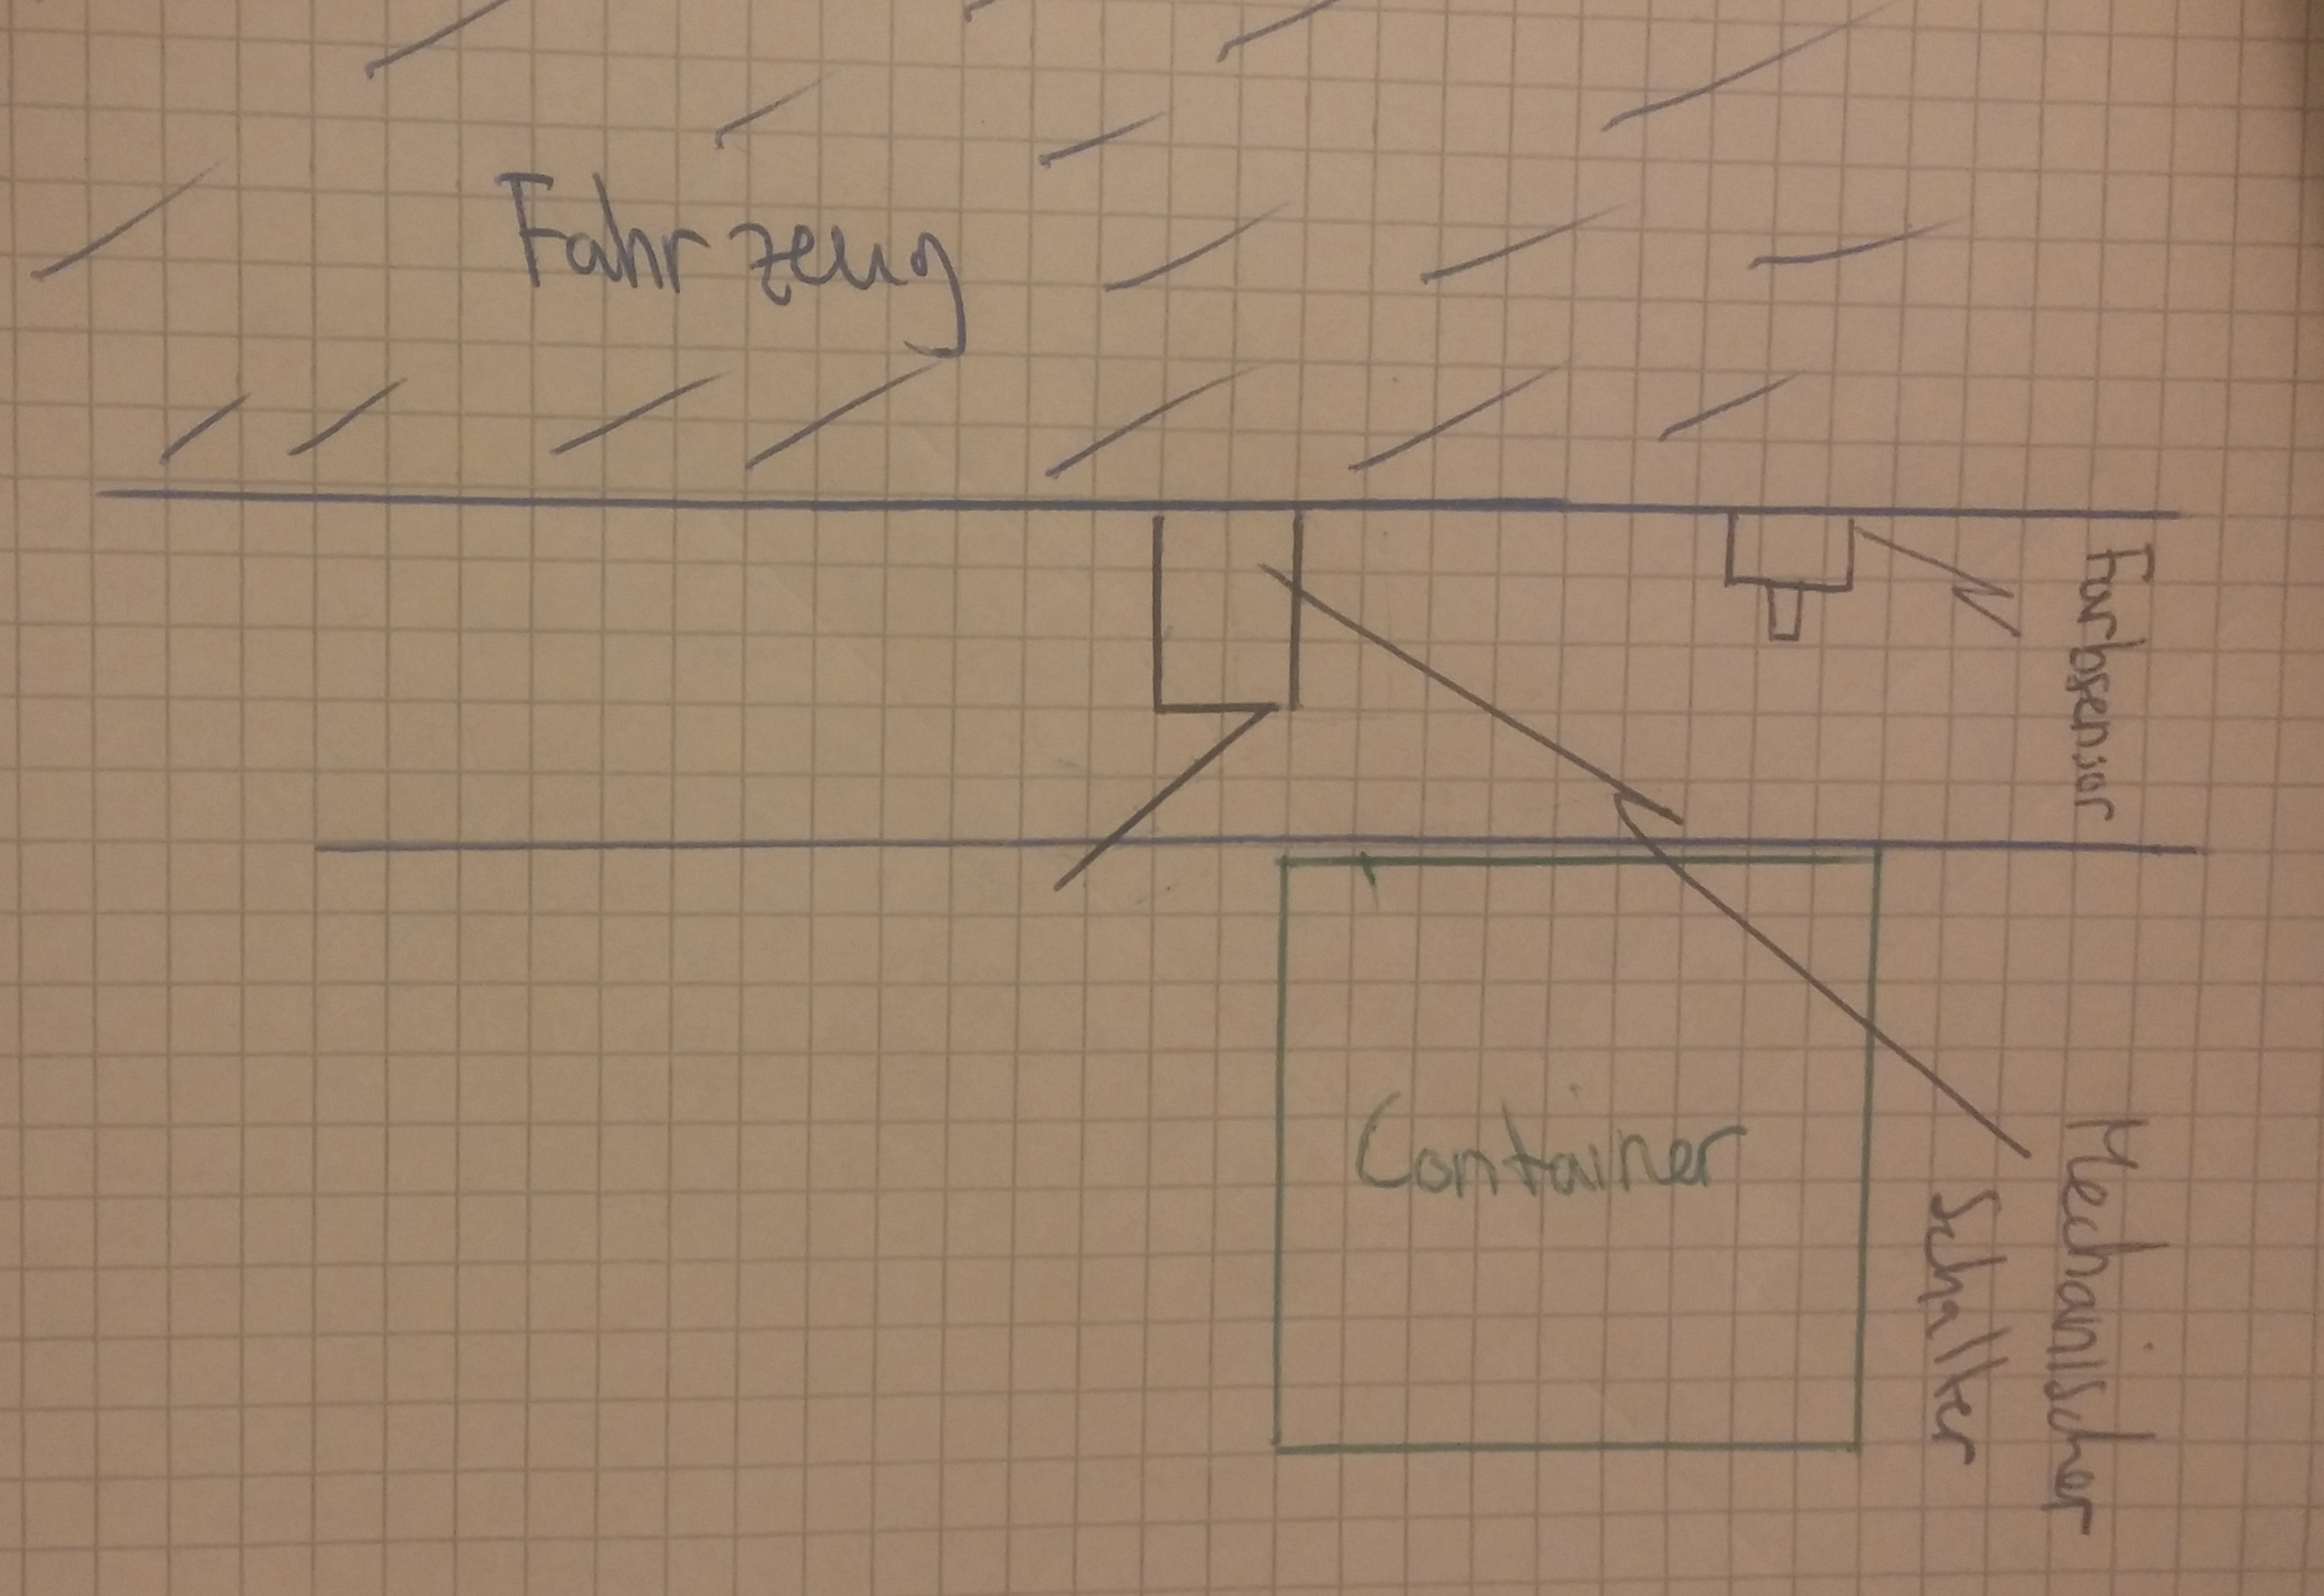
\includegraphics[width=0.5\textwidth]{Images/Containererkennung_1.png}
	\caption{Distanzsensoren an der rechten Seite des Fahrzeugs}
\end{figure}

\textbf {Mechanische Detektion und Farbsensoren}
\begin{itemize}
\item Unbekannte Genauigkeit muss getestet werden.
\item Klarer Wert
\item Mechanischer Kontakt (darf nichts ausser den Container berühren)
\end{itemize}
\begin{figure} [hbp]
	\centering
	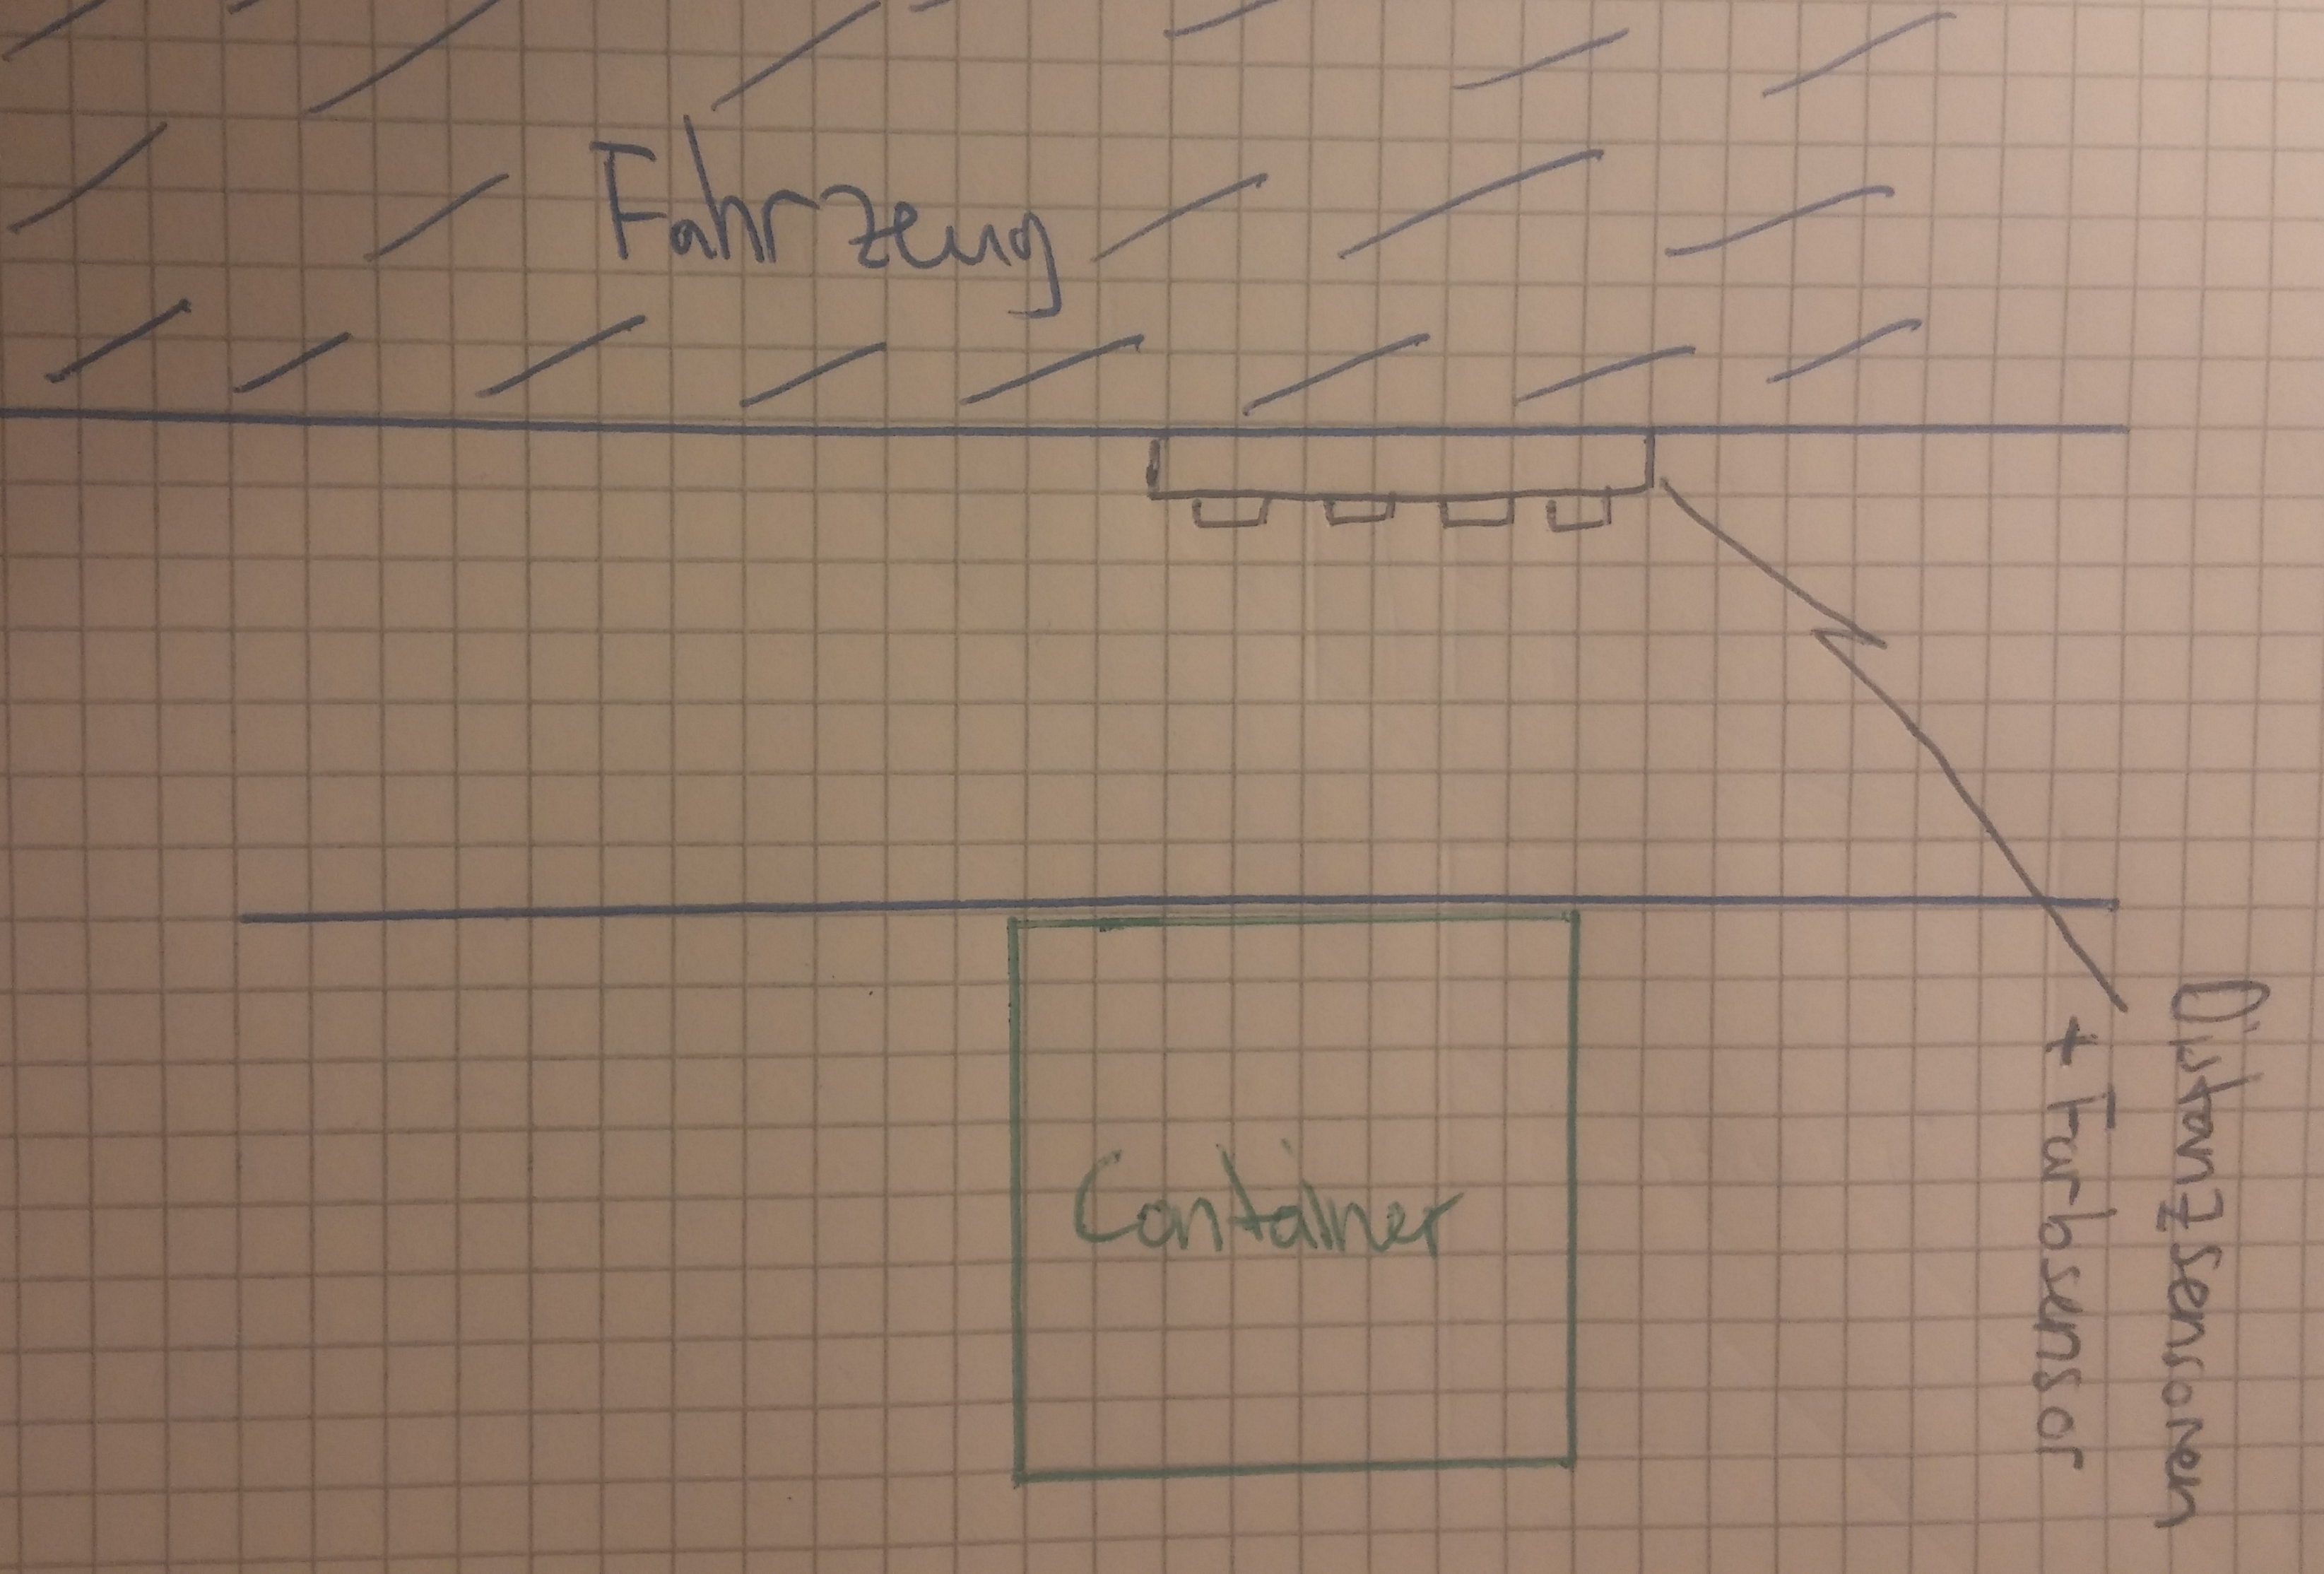
\includegraphics[width=0.5\textwidth]{Images/Containererkennung_2.png}
	\caption{Ein Schalter an der rechten Seite des Fahrzeugs}
\end{figure}
\subsection{2}
\subsection{3}